\documentclass[12pt]{article}

\usepackage[utf8]{inputenc}
\usepackage{graphicx} % Required for the inclusion of images
\usepackage{amsmath} % Required for some math elements 
\usepackage{float} % to pose images with H parameter
\usepackage{subfig}

%----------------------------------------------------------------------------------------
%	DOCUMENT INFORMATION
%----------------------------------------------------------------------------------------

\title{\textbf{Macchinetta per caffè macchiato}} % Title
\author{Moreno Bragaglio} % Author name
\date{\today} % Date for the report
\begin{document}

% ------------- HEADING PAGE
\maketitle % Insert the title, author and date
\begin{center}
\begin{tabular}{l r}
Instructors: \\
& Professor Tiziano Villa \\
& Assistant Professor Luca Geretti
\end{tabular}
\end{center}
\newpage
\tableofcontents

\newpage
\begin{abstract}
Il sistema analizzato si riferisce a una macchina da caffè. In particolare si vuole riempire una tanica con 6 cl di caffè e successivamente 4 cl di schiuma derivante da latte. Saranno descritti gli automi, usati per rappresentare tutto il sistema. La composizione degli automi utilizza la formula controllore/attuatore nella quale le valvole fungono da attuatori e vengono gestite da un controllore.
I risultati sono rappresentati da grafici che descrivono l'andamento del livello dei liquidi nelle varie taniche durante l'evoluzione del sistema. \\
Particolare importanza è anche data all'analisi delle difficoltà riscontrate. A tal fine, verrà scritta una sezione speciale. Per ogni difficoltà verrà esposta la soluzione raggiunta.\\
Per sviluppare il tutto si ha utilizzato la libreria Ariadne scritta in C++ [vedere link in bibliografia].
\end{abstract}


%----------------------------------------------------------------------------------------
%	SECTION 1
%----------------------------------------------------------------------------------------
\newpage
\section{Definition of the system}
Il sistema rappresentato consiste in 4 taniche e 6 valvole ed è descritto come segue:
\begin{figure}[H]
\begin{center}
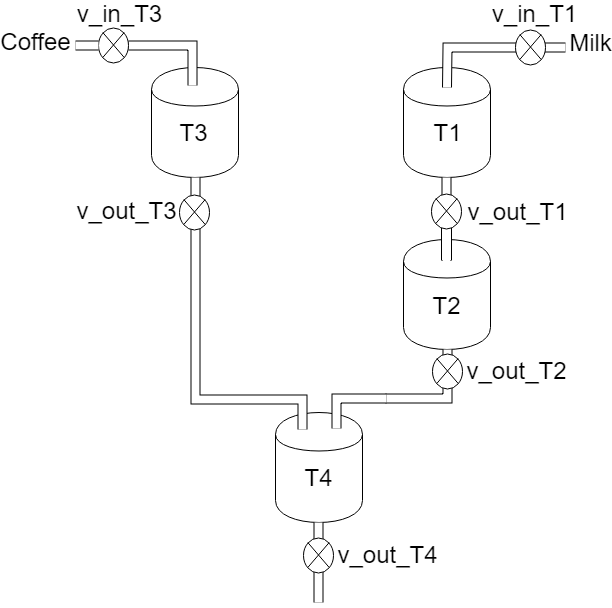
\includegraphics[width=0.65\textwidth]{images/system.png} % Include the image placeholder.png
\caption{System}
\end{center}
\end{figure}

\subsection{Funzionamento generale}
Il funzionamento generale prevede che nella tanica T1 entri del latte freddo il quale viene scaldato nella tanica T1 stessa. Successivamente tale latte passa nella tanica T2 nella quale si simula la conversione del latte in schiuma. Nel frattempo la tanica T3 contiene un livello sempre costante di caffè. Nella tanica T4 quindi viene inserito prima di tutto il caffè della tanica T3 e successivamente, una volta che il livello di caffè in T4 è sufficiente, viene aggiunta la schiuma derivante dalla tanica T2.

\subsection{Funzionamento nel dettaglio}
Andando più nel dettaglio si espone di seguito il funzionamento del sistema analizzando interconnessione tra valvole e taniche.\\
Inizialmente le valvole del sistema si trovano nella seguente configurazione:
\begin{itemize}
	\item \textit{valvola v\_in\_t1}: aperta
	\item \textit{valvola v\_out\_t1}: chiusa
	\item \textit{valvola v\_out\_t2}: chiusa
	\item \textit{valvola v\_in\_t3}: chiusa
	\item \textit{valvola v\_out\_t3}: chiusa
	\item \textit{valvola v\_out\_t4}: chiusa
\end{itemize}  
Tutte le valvole implementano un comportamento ad isteresi. Esse quindi si aprono e chiudono con una variazione di apertura pari ad $1/T$ dove $T$ è una costante.

\subsection{Tanica T1}
La tanica T1 è inizializzata con 2 (si suppone ad esempio che l'unità di misura siano cl) già presenti al suo interno. La si riempirà fino ad un totale di 4cl. A tal punto la valvola v\_in\_t1 comincia a chiudersi fino a raggiungere la chiusura totale. \\
In definitiva, dopo i suddetti passaggi, 4 cl di latte si trovano nella tanica T1 e son pronti per passare nella tanica T2. Le valvole v\_in\_t1 e v\_out\_t1 sono chiuse.\\
Si noti che il riscaldamento del latte viene idealizzato supponendolo immediato una volta completato il riempimento della tanica T1.\\\\
La formula che calcola la variazione di livello di latte nella tanica 1 è:
\begin{center}
	$ \dot{height\_T1} = aperture\_v\_in\_t1*rate - aperture\_v\_out\_t1*rate$
\end{center}
Se la derivata è positiva significa che il livello di latte aumenta, se è negativa allora diminuisce, se è nulla allora rimane invariato.\\
Il parametro \textit{rate} serve per simulare la pressione nel tubo in cui passa il latte.


\subsection{Tanica T2}
Inizialmente la tanica T2 è vuota. Una volta che la valvola v\_in\_t1 si è chiusa del tutto, può cominciare ad aprirsi la valvola v\_out\_t1 dando inizio allo svuotamento della tanica T1 e al riempimento della tanica T2. Successivamente, quando tutti i cl della tanica T1 son passati nella tanica T2, la valvola v\_out\_t1 viene chiusa.\\
In definitiva, dopo i suddetti passaggi, i 4 cl di latte caldo si trovano nella tanica T2 e vengon convertiti in schiuma. La schiuma è quindi pronta per passare nella tanica T4 quando sarà possibile.\\
Si noti che la conversione da latte caldo a schiuma è idealizzata supponendola immediata una volta completato il riempimento della tanica T2. Inoltre la conversione in schiuma si suppone non generi un aumento ne di volume ne di cl. \\\\
La formula che calcola la variazione di livello di latte nella tanica 2 è:
\begin{center}
$ \dot{height\_T2} = aperture\_v\_out\_t1*rate - aperture\_v\_out\_t2*rate$
\end{center}
Per simulare la viscosità della schiuma confronto a quella del latte si è usata la seguente strategia:
l'incremento di livello, della tanica T4, con schiuma, viene incrementato più lentamente. Per far ciò si è passati ad un valore della costante $T$ più alto per la valvola v\_out\_t2. Tale valore infatti influenza la velocità di apertura della valvola che quindi farà passare la schiuma in un tempo maggiore confronto ad un passaggio di latte.


\subsection{Tanica T3}
La tanica T3 ha un funzionamento molto semplice. Inizialmente è vuota. Il livello di caffè in essa contenuto vien sempre mantenuto costante. Per fare ciò si è implementato un comportamento che consiste nell'apertura e chiusura contemporanea delle valvole v\_in\_t3 e v\_out\_t3, in tal modo il caffè uscente da T3 è compensato da quello entrante.
La formula che calcola la variazione di livello di caffè nella tanica 3 è:
\begin{center}
$ \dot{height\_T3} = aperture\_v\_in\_t3*rate - aperture\_v\_out\_t3*rate$
\end{center}

\subsection{Tanica T4}
La tanica T4 viene inizializzata vuota. Prima di tutto vengono versati 6 cl di caffè tramite l'apertura della valvola v\_out\_T3. Una volta raggiunto tale livello la valvola v\_out\_T3 vien chiusa. Quando nella tanica T2 saranno disponibili 4 cl di schiuma essi verranno versati nella tanica T4 attraverso l'apertura della valvola v\_out\_T2. Si noti che si possono versare i 4 cl di schiuma se e solo se nella tanica T4 son già stati versati i 6 cl di caffè.\\ Una volta quindi che in T4 sono presenti $6+4=10 cl$ di liquidi, T4 viene svuotata completamente. Si suppone che lo svuotamento sia immediato come se avvenisse un cambio di T4 con un'altra tanica.

\subsection{Valvola v\_in\_T1}
\begin{itemize}
	\item \textit{Apertura}: si apre quando la tanica T1 è vuota e la valvola v\_out\_T1 è completamente chiusa. Si noti che durante lo svuotamento di T1 il livello di latte al suo interno cala ma ciò non deve causare apertura della valvola v\_in\_t1 al fine di ristabilire i 4 cl in T1. Questo è dovuto al fatto che altrimenti non avrei più la gestione totale di 4 cl di latte ma di una quantità maggiore andando quindi contro le specifiche.
	\item \textit{Chiusura}: resta chiusa quando nella tanica T1 son già presenti i 4 cl di latte. 
\end{itemize}

\subsection{Valvola v\_out\_T1}
\begin{itemize}
	\item \textit{Apertura}: si apre solo quando nella tanica T1 sono presenti i 4 cl di latte e le valvole v\_in\_T1 e v\_out\_T2 sono chiuse del tutto.
	\item \textit{Chiusura}: si chiude solo quando nella tanica T2 vengon versati tutti i 4 cl della tanica T1 
\end{itemize}
	
\subsection{Valvola v\_out\_T2}
\begin{itemize}
	\item \textit{Apertura}: si apre solo quando nella tanica T2 sono presenti i 4 cl di schiuma e nella tanica T4 son già presenti i 6 cl di caffè derivanti dalla tanica T3.
	\item \textit{Chiusura}: si chiude quando il livello di T4 supera i 10 cl.
\end{itemize}
	
\subsection{Valvola v\_in\_T3}
\begin{itemize}
	\item \textit{Apertura}: si apre nello stesso istante in cui si apre la valvola v\_out\_T3
	\item \textit{Chiusura}: si chiude nello stesso istante in cui si chiude la valvola v\_out\_T3
\end{itemize}

\subsection{Valvola v\_out\_T3}
\begin{itemize}
	\item \textit{Apertura}: si apre quando la tanica T4 è vuota.
	\item \textit{Chiusura}: si chiude quando la tanica T4 raggiunge un livello di caffè pari a 6 cl.
\end{itemize}
	
\subsection{Valvola v\_out\_T4}
\begin{itemize}
	\item \textit{Apertura}: si apre se e solo se nella tanica T4 si hanno almeno 10 cl di liquido. Questa è l'unica valvola che non segue il comportamento ad isteresi. L'apertura è quindi immediata facendo svuotare istantaneamente la tanica T4.
	
	\item \textit{Chiusura}: rimane chiusa se e solo se nella tanica T4 si hanno meno di 10 cl di liquido.
\end{itemize}



%----------------------------------------------------------------------------------------
%	SECTION 2
%----------------------------------------------------------------------------------------
\newpage
\section{Automi per la descrizione del sistema}
Vengono di seguito riportati gli automi necessari per il funzionamento del sistema. Si noti che l'implementazione utilizza una costante $\delta$ in modo tale da simulare la gestione di rumore che potrebbe affliggere il sistema.
\begin{itemize}
	\item \textbf{Controller 1}
	\begin{figure}[H]
	\begin{center}
	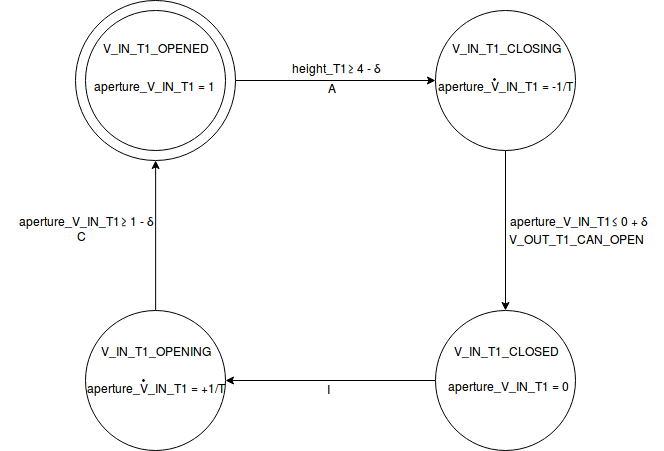
\includegraphics[width=1\textwidth]{images/controller1.png}
	\end{center}
	\end{figure}
	
	\newpage
	\item \textbf{Controller 2}
	\begin{figure}[H]
	\begin{center}
	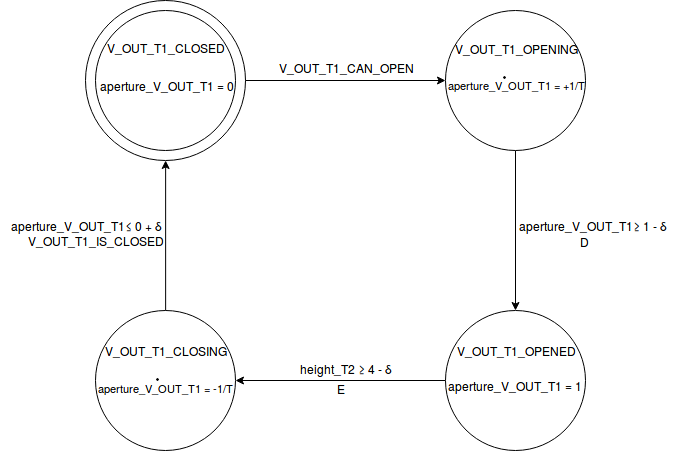
\includegraphics[width=1\textwidth]{images/controller2.png}
	\end{center}
	\end{figure}
	
	\newpage
	\item \textbf{Controller 3}
	\begin{figure}[H]
	\begin{center}
	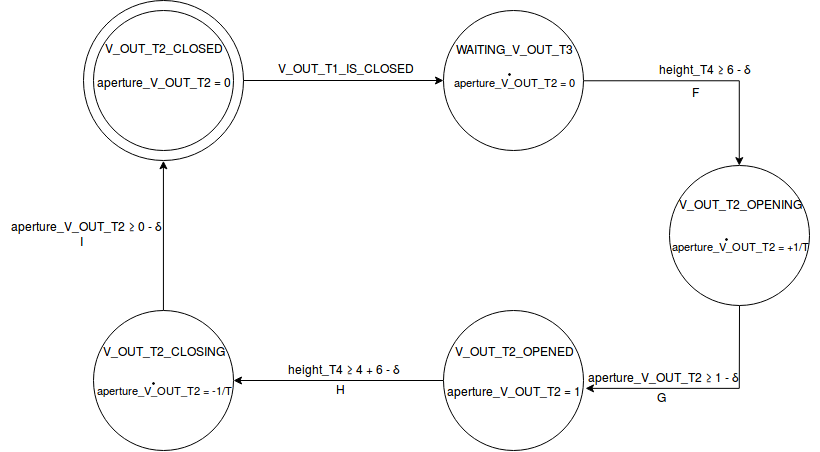
\includegraphics[width=1\textwidth]{images/controller3.png}
	\end{center}
	\end{figure}
	
	\newpage
	\item \textbf{Controller 4}
	\begin{figure}[H]
	\begin{center}
	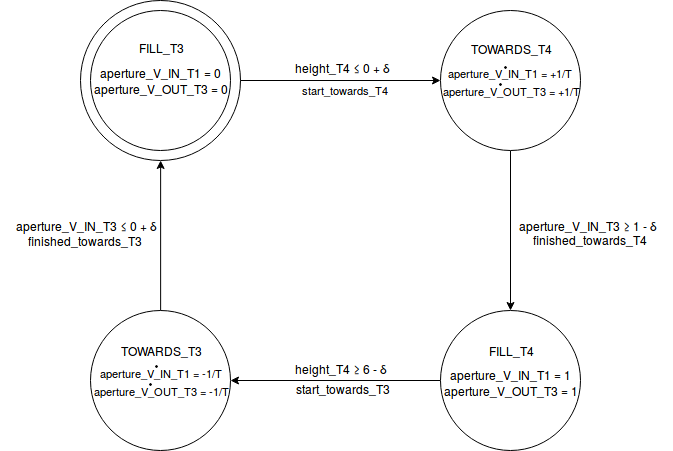
\includegraphics[width=1\textwidth]{images/controller4.png}
	\end{center}
	\end{figure}
	
	\item \textbf{Controller 5}
	\begin{figure}[H]
	\begin{center}
	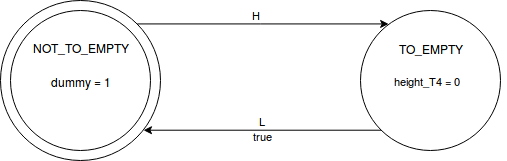
\includegraphics[width=0.8\textwidth]{images/controller5.png}
	\end{center}
	\end{figure}
	
	\newpage
	\item \textbf{Tank 1}
	\begin{figure}[H]
	\begin{center}
	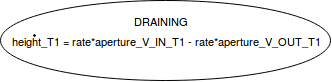
\includegraphics[width=0.65\textwidth]{images/tank1.png}
	\end{center}
	\end{figure}
	
	\item \textbf{Tank 2}
	\begin{figure}[H]
	\begin{center}
	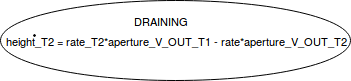
\includegraphics[width=0.65\textwidth]{images/tank2.png}
	\end{center}
	\end{figure}
	
	\item \textbf{Tank 3}
	\begin{figure}[H]
	\begin{center}
	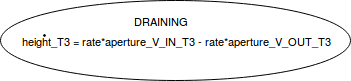
\includegraphics[width=0.65\textwidth]{images/tank3.png}
	\end{center}
	\end{figure}
	
	\item \textbf{Tank 4}
	\begin{figure}[H]
	\begin{center}
	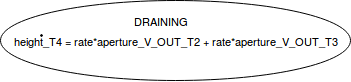
\includegraphics[width=0.65\textwidth]{images/tank4.png}
	\end{center}
	\end{figure}
\end{itemize}


%----------------------------------------------------------------------------------------
%	SECTION 3
%----------------------------------------------------------------------------------------
\newpage
\section{Problematiche riscontrate}
Si riporta di seguito un elenco delle maggiori difficoltà riscontrate durante lo sviluppo del progetto.
\begin{itemize}
	\item \textit{Problematica 1}\\
	Si supponga di avere uno stato B all'interno del quale si ha un'equazione differenziale. \\
	La difficoltà è stata nel comprendere che quando si effettua una transazione da uno A a tale stato B, la transazione deve contenere il comando \textit{next} in modo da specificare il nuovo stato iniziale della variabile derivata nell'equazione differenziale. \\
	Si è capito infatti che ad ogni iterazione bisogna sempre definire il valore delle variabili altrimenti queste è come se non fossero gestite. In particolare non bisogna quindi pensare che se una variabile non viene utilizzata in un certo stato allora essa mantiene l'ultimo valore che le è stato assegnato; Se una variabile viene creata, bisogna poi, ad ogni iterazione, gestirla dicendo quale è il suo valore futuro utilizzando appunto il comando \textit{next}.
	
	\item \textit{Problematica 2}\\
	Si supponga di avere due automi A1 e A2 che comunicano tra loro. In particolare si supponga che l'automa A genera un messaggio X su una sua guardia e l'automa A2 ha una transizione che scatta nel momento in cui viene appunto generato il messaggio X. In pratica è un classico comportamento \textit{"Event Driven"} per sincronizzare tra loro A1 e A2.\\
	Può capitare che Ariadne dia errore malgrado la sincronizzazione logicamente sia corretta. Questo perchè il sistema può evolvere in modo tale che il messaggio X viene generato quando A2 si trova su uno stato differente da quello desiderato (stato di ascolto dell'automa A2.\\
	Di conseguenza si è obbligati a specificare per ogni stato dell'automa A1 la transazione con messaggio X, ma con una guardia falsa, in modo che tale transazione non possa mai capitare. In tal modo l'automa A2 potrà ricevere il messaggio X solamente dallo stato desiderato dell'automa A1 e mai da altri.\\
	Tutto ciò serve a far si che il sistema sia un \textit{"sistema chiuso"} cioè si vuole cercare di avere sempre sottocontrollo l'evoluzione in modo da limitare al massimo la possibilità di errore.
	
	\item \textit{Problematica 3}\\
	Alcune difficoltà sono sorte anche dalla non sempre semplice interpretazione dei messaggi d'errore restituiti da Ariadne. Non è sempre stato facile interpretarli al fine di capire quale effettivamente fosse l'errore. Spesso tali messaggi erano sottoforma di codice piuttosto che in linguaggio umano. Di fatto ciò ha reso poco comprensibile, a chi non ha scritto la libreria Ariadne, il motivo dell'errore in esame.	
	
\end{itemize}



%----------------------------------------------------------------------------------------
%	SECTION 4
%----------------------------------------------------------------------------------------
\newpage
\section{Risultati e Conclusioni}
Il sistema è analizzabile attraverso l'esame dei seguenti grafici che rappresentano la variazione del livello nelle determinate taniche nel corso del tempo.
\begin{figure}[H]
\begin{center}
	\subfloat[Tanica T1]{
		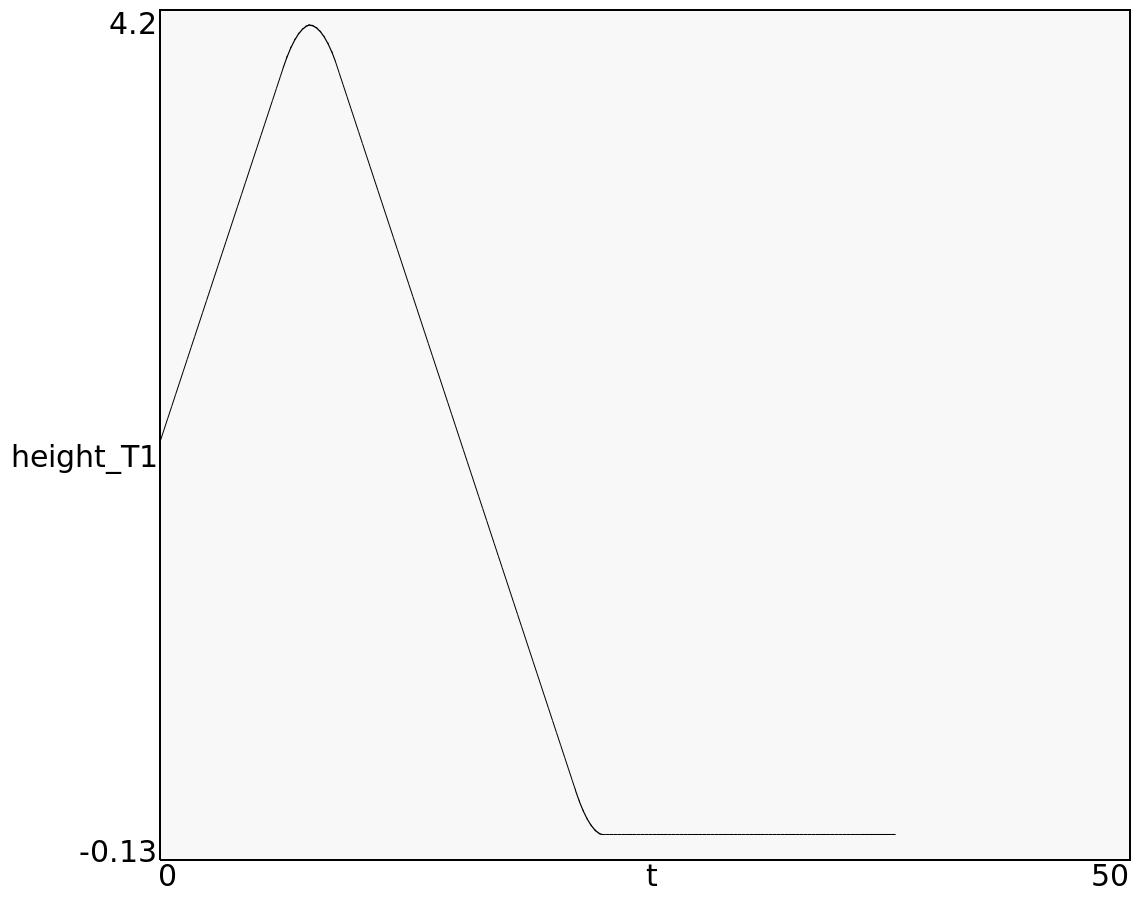
\includegraphics[width=0.4\textwidth]{images/graph_tank1.png}
	}
	
	\subfloat[Tanica T2]{
		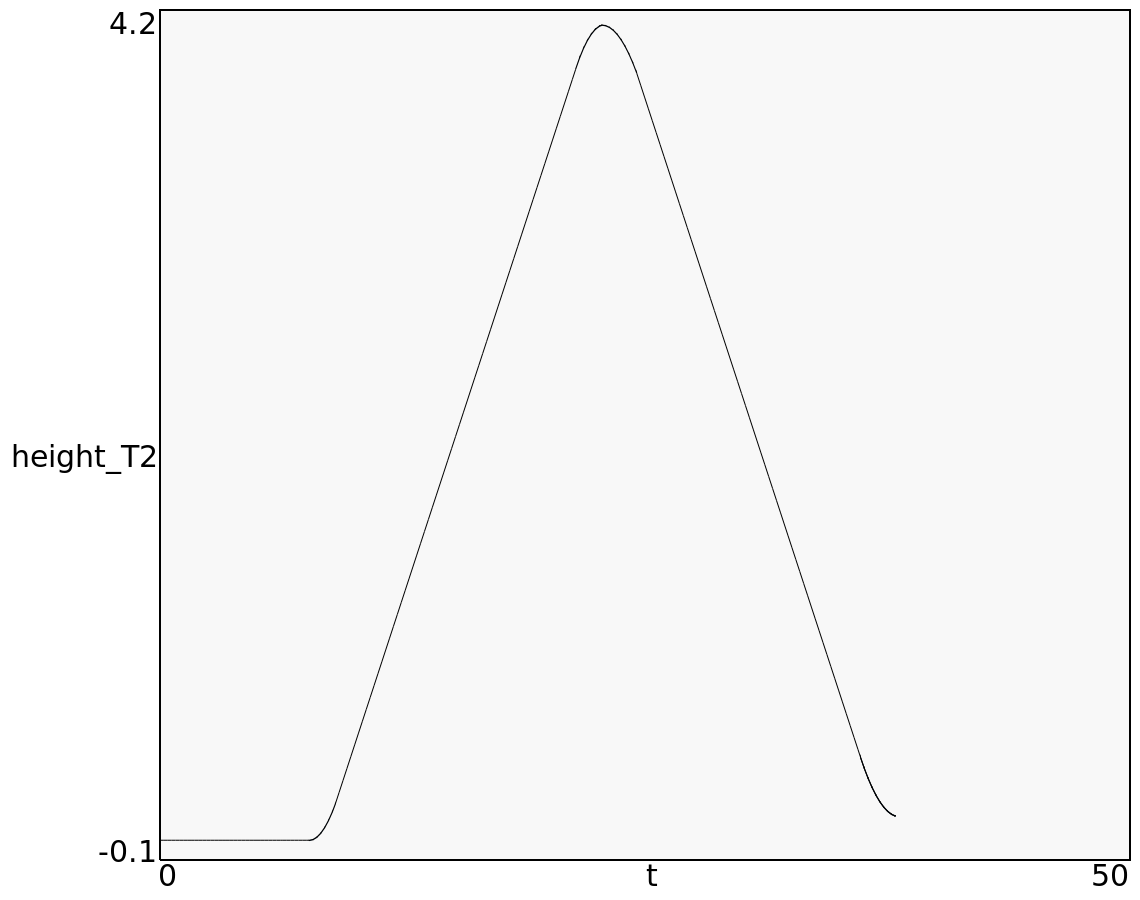
\includegraphics[width=0.40\textwidth]{images/graph_tank2.png}
	}
	
	\subfloat[Tanica T4]{
		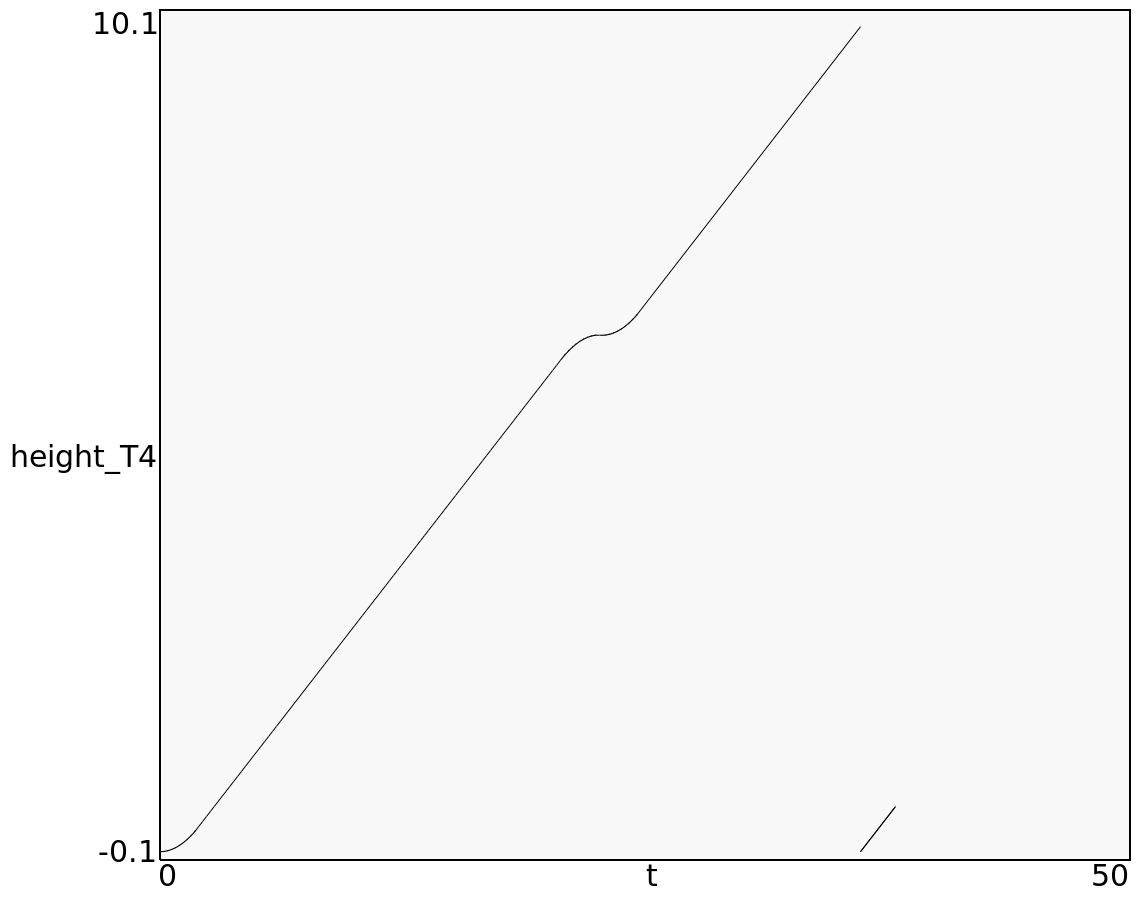
\includegraphics[width=0.40\textwidth]{images/graph_tank4.png}
	}
	\caption{Livello nelle taniche durante l'evoluzione del sistema}
\end{center}
\end{figure}
	Da tale grafico si nota che la tanica T1 inizialmente già contiene una certa quantità di latte (2 cl) e che quindi si riempie fino a 4 cl (valvola v\_in\_T1 aperta). Nel momento in cui è piena la valvola v\_in\_T1 comincia a chiudersi fino alla completa chiusura (punto di massimo globale nel grafico della tanica T1). \\
Successivamente comincia ad aprirsi la valvola v\_out\_T1 e di conseguenza, nello stesso istante, comincia a riempirsi la tanica T2. Come si vede anche dai grafici, quando T1 si svuota del tutto T2 si riempie del tutto. Da qui in poi T1 rimarrà vuota finchè non verrà chiusa del tutto la valvola v\_out\_T2.
Nel momento in cui la tanica T2 è piena, la valvola v\_out\_T1 comincia a chiudersi fino a raggiungere la chiusura totale.\\
Durante il corso di tutto il procedimento descritto, la tanica T4 si è riempita di caffè tramite l'apertura della valvola v\_out\_T3 fino al raggiungimento di un livello pari a 6 cl. Una volta raggiunto tale livello la valvola v\_out\_T3 si chiude fino a completa chiusura. Dal grafico si vede che quando in T4 ci sono i 6 cl, si ha un momento di stallo in attesa che la tanica T2 sia piena. Infatti quando poi la tanica T2 si riempie completamente essa comincia a svuotarsi tramite l'apertura della valvola v\_out\_T2 e conseguentemente si ha il proseguo di riempimento della tanica T4. Quando la tanica T4 raggiunge i 10 cl significa che la tanica T2 si è svuotata del tutto. Ciò è visibile dai grafici nei quali appunto l'istante di svuotamento totale di T2 e riempimento totale di T4 combaciano.\\
Si vede poi che T4 si svuota istantaneamente in accordo con l'automa \textit{controller 5}. In seguito T4 riprenderebbe a riempirsi di caffè e il ciclo ricomincerebbe da capo.
\begin{figure}[H]
\begin{center}
	\subfloat[Tanica T3]{
		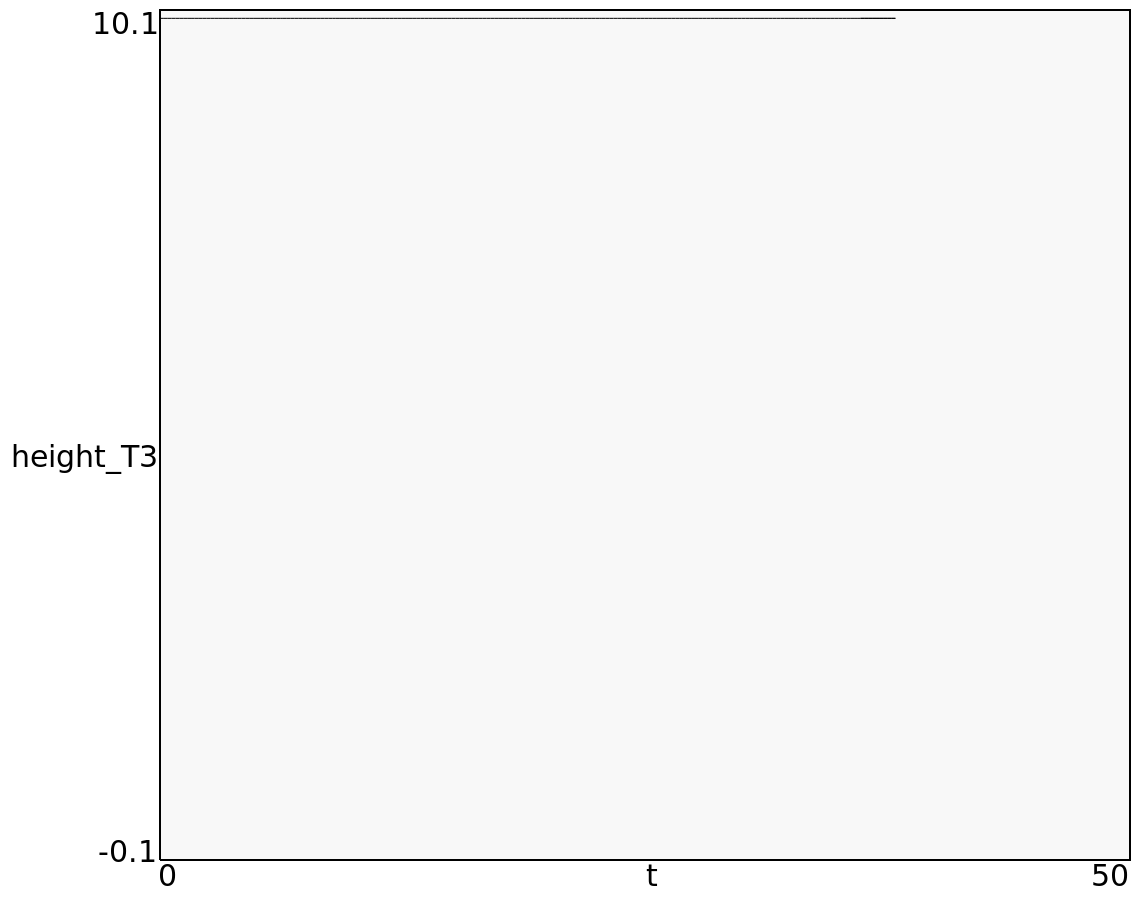
\includegraphics[width=0.45\textwidth]{images/graph_tank3.png}
	}
	\caption{Livello nella tanica T3 durante l'evoluzione del sistema}
\end{center}
\end{figure}
Infine si noti che, in accordo con l'automa \textit{controller 4} la tanica T3 mantiene il suo livello di caffè costante. Infatti, durante l'evoluzione del sistema, se si apre la valvola v\_out\_T3 per riempire la tanica T4, in contemporanea si apre anche la valvola v\_in\_T3. Stesso discorso per la fase di chiusura.\\\\
In conclusione si è riusciti a rappresentare il sistema desiderato tramite la libreria Ariadne. Una versione scaricabile di tale progetto è presente su GitHub nel link lasciato nella bibliografia.




%----------------------------------------------------------------------------------------
%	BIBLIOGRAPHY
%----------------------------------------------------------------------------------------
\newpage
\Large{\textbf{Sitografia}}\\
\begin{itemize}  
\item Sito Ariadne: http://www.ariadne-cps.org/
\item Link download progetto: https://github.com/MorenoBragaglio/caffe
\end{itemize}
%----------------------------------------------------------------------------------------


\end{document}